\documentclass[a4paper,12pt]{article}

\usepackage [utf8x] {inputenc} %кодировка исходного текста
\usepackage [T2A] {fontenc} %кодировка
\usepackage [english, russian] {babel}
\usepackage{color}
\usepackage{amsmath, amsfonts, amssymb, amsthm, mathtools}
\usepackage{graphicx}
\graphicspath{{.}}
\DeclareGraphicsExtensions{.pdf,.png,.jpg}
\righthyphenmin=2


\title{Лабораторная работа 0}
\author{Калашников Михаил, Б03-205}
\date{}


\begin{document}

\maketitle{Арифметика и основы работы с листингами}

\begin{enumerate}

\setcounter{enumi}{0}

\item А я поставил WSL.

\item И установил g++.

\item Написал helloworld и сгенерировал листинг с помощью флага -S (рис. 1).

\item Сгенерируем листинг для программы, складывающей два числа. В листинге изменим значение одной из переменных. Скомпилируем результат и получим другой вывод (рис. 2).

\item Напишем helloworld на C и сравним с листингом из пункта 3. Листинг выглядит гораздо проще и компактнее (рис. 3). Для пункта 4 получает аналогичный результат.

\item Добавим в код операцию вычитания и определим, что за присвоение отвечает команда mov, за сложение -- add, а за вычитание -- sub (рис. 4).

\item Объявим три глобальные переменные типов int (a = 1), float (b = 2.5) и char (c = '0'). Найдем их объявление в листинге (рис. 5). В int записывается ее же численное значение, в char индекс символа в ASCII, а вот с float не очень понятно. Похоже, что он переводит число с плавающей точкой в целое число и хранит уже целочисленное значение.

\item Регистрами общего назначения являются регистры eax, edx, ecx и ebx. Их размер составляет 4 байта. Так же существуют расширенные регистры rax, rdx, rcx и rbx, имеющие размер 8 байт. Вызываются они с помощью \%(название регистра). Например, команда "movl	\%eax, \%edx" переложит содержимое регистра eax в регистр edx.

\item Команда mul отвечает за умножение беззнаковых переменных, а imul за умножение знаковых. Команды div/idiv работают аналогично, только отвечают уже за деление. Это написано в интернете. На деле же отличие заключается в том, что команда mul принимает только один аргумент, а второй множитель берет из регистра eax (рис. 6). Знак переменных на работу функции никак не влияет. idiv и div принимают только один аргумент -- делитель, делимое они берут из регистра eax. idiv работает с целочисленными значениями любого знака, а div -- только с положительными.

\end{enumerate}

\section*{Приложения}

\begin{figure}[h]
  \centering
  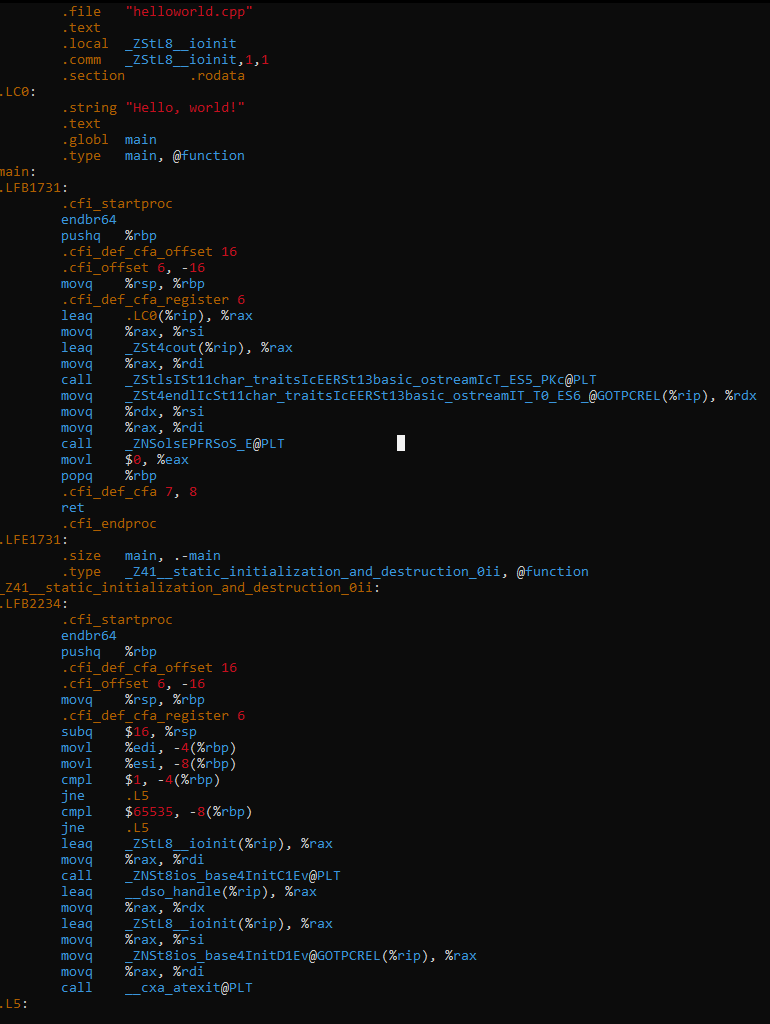
\includegraphics[width=0.8\linewidth]{images/asm0_0.png}
  \caption{Ассемблерный листинг helloworld.cpp}
\end{figure}

\begin{figure}[h]
  \centering
  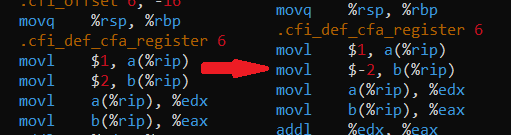
\includegraphics[width=0.8\linewidth]{images/asm0_1.png}
  \caption{Изменение листинга}
\end{figure}

\begin{figure}[h]
  \centering
  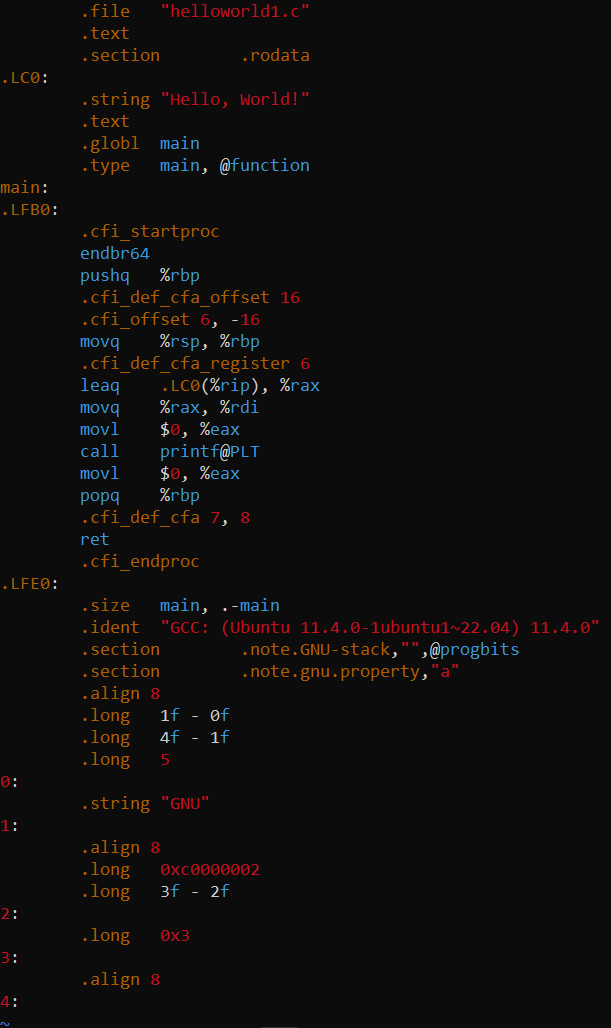
\includegraphics[width=0.8\linewidth]{images/asm0_2.png}
  \caption{Листинг helloworld на C}
\end{figure}

\begin{figure}[h]
  \centering
  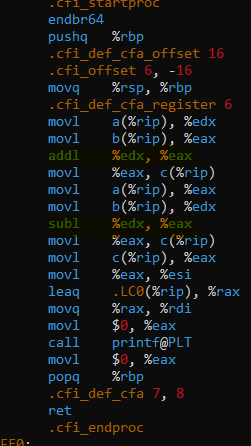
\includegraphics[width=0.8\linewidth]{images/asm0_3.png}
  \caption{Сложение и вычитание}
\end{figure}

\begin{figure}[h]
  \centering
  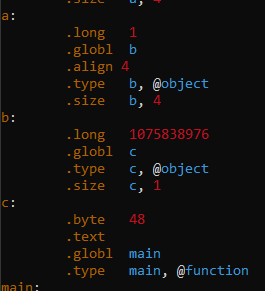
\includegraphics[width=0.8\linewidth]{images/asm0_4.png}
  \caption{Глобальные переменные различных типов}
\end{figure}

\begin{figure}[h]
  \centering
  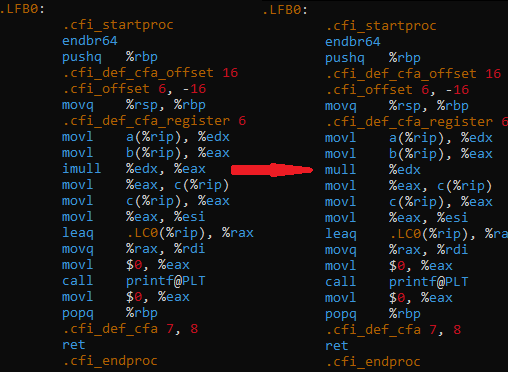
\includegraphics[width=0.8\linewidth]{images/asm0_5.png}
  \caption{Замена imul на mul}
\end{figure}

\end{document}